\section{QCD estimation using the transverse W mass distribution}
\label{sec:qcdWithWmT}
As there are not enough Monte Carlo events passing the selection; 
the sideband samples, which mirror the QCD background, are used
instead. Specifically, we invert the lepton isolation to be $>0.1$
(default selection uses Iso$_{mu}<0.1$ and Iso$_{el}<0.05$). 
We also relax the MET cut to $>20GeV$ and (for electrons) the ID  
requirement to $WP90$-like. 
The $W_{mT}$ distributions from the Data and MC are
statistically consistent, as shown in Figure~\ref{fig:QCDCutLooseningWmT}
for muons (for electrons there's an insufficient amount of MC events
to make the comparison). 
On the other hand, relying on data sidebands provides a
sufficient amount of events to construct the templates. 


Since the
$W_{mT}$ distribution is the same for all processes except
QCD, we perform a fit to the data using the W$jj$ and QCD
templates - Figure~\ref{fig:QCDTemplateFitWmT} (with MET$>20$~GeV, in order to
take full advantage of available statistics) and fix the fraction of
QCD relative to the data. 
After accounting for the acceptances the corresponding fractions are: 
$\mu_{2J}$ $frac_{QCD}=0.028\pm 0.009$, $el_{2J}$ $frac_{QCD}=0.087\pm 0.007$, $\mu_{3J}$ $frac_{QCD}=0.081\pm 0.021$, $el_{3J}$ $frac_{QCD}=0.099\pm 0.011$.
%%%%%%%%%%%%%%%%%%%%%%%%%%%%
%%%%%%%
\begin{figure}[h!] {\centering
\unitlength=0.33\linewidth
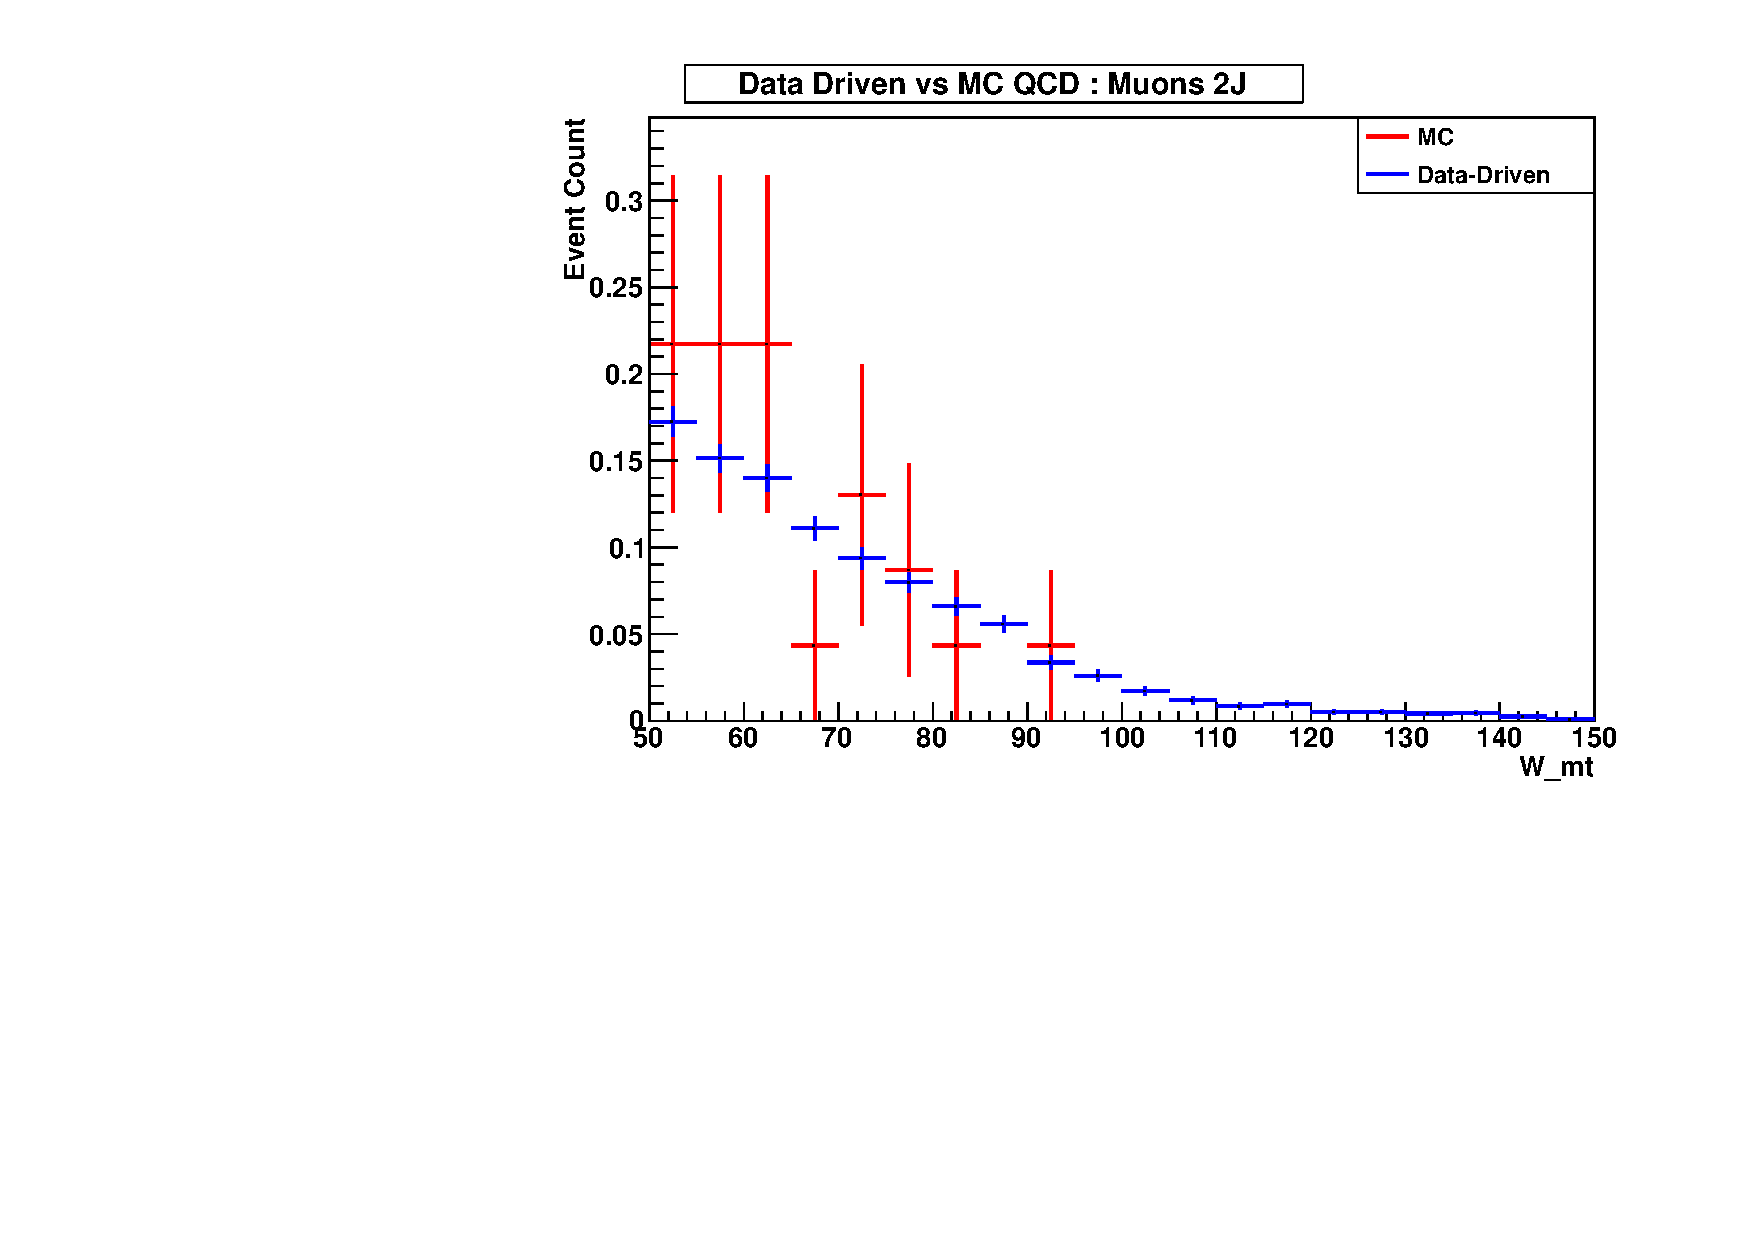
\includegraphics[width=0.48\textwidth]{figs/QCDDataVSMC_Muons2J.pdf}
\caption{ Comparison of the $W_{mT}$ shapes for MC vs Data-Driven QCD events. The two are statistically consistent.} 
\label{fig:QCDCutLooseningWmT}}
\end{figure}
%%%%%%%
%%%%%%%
\begin{figure}[h!] {\centering
%\unitlength=0.33\linewidth
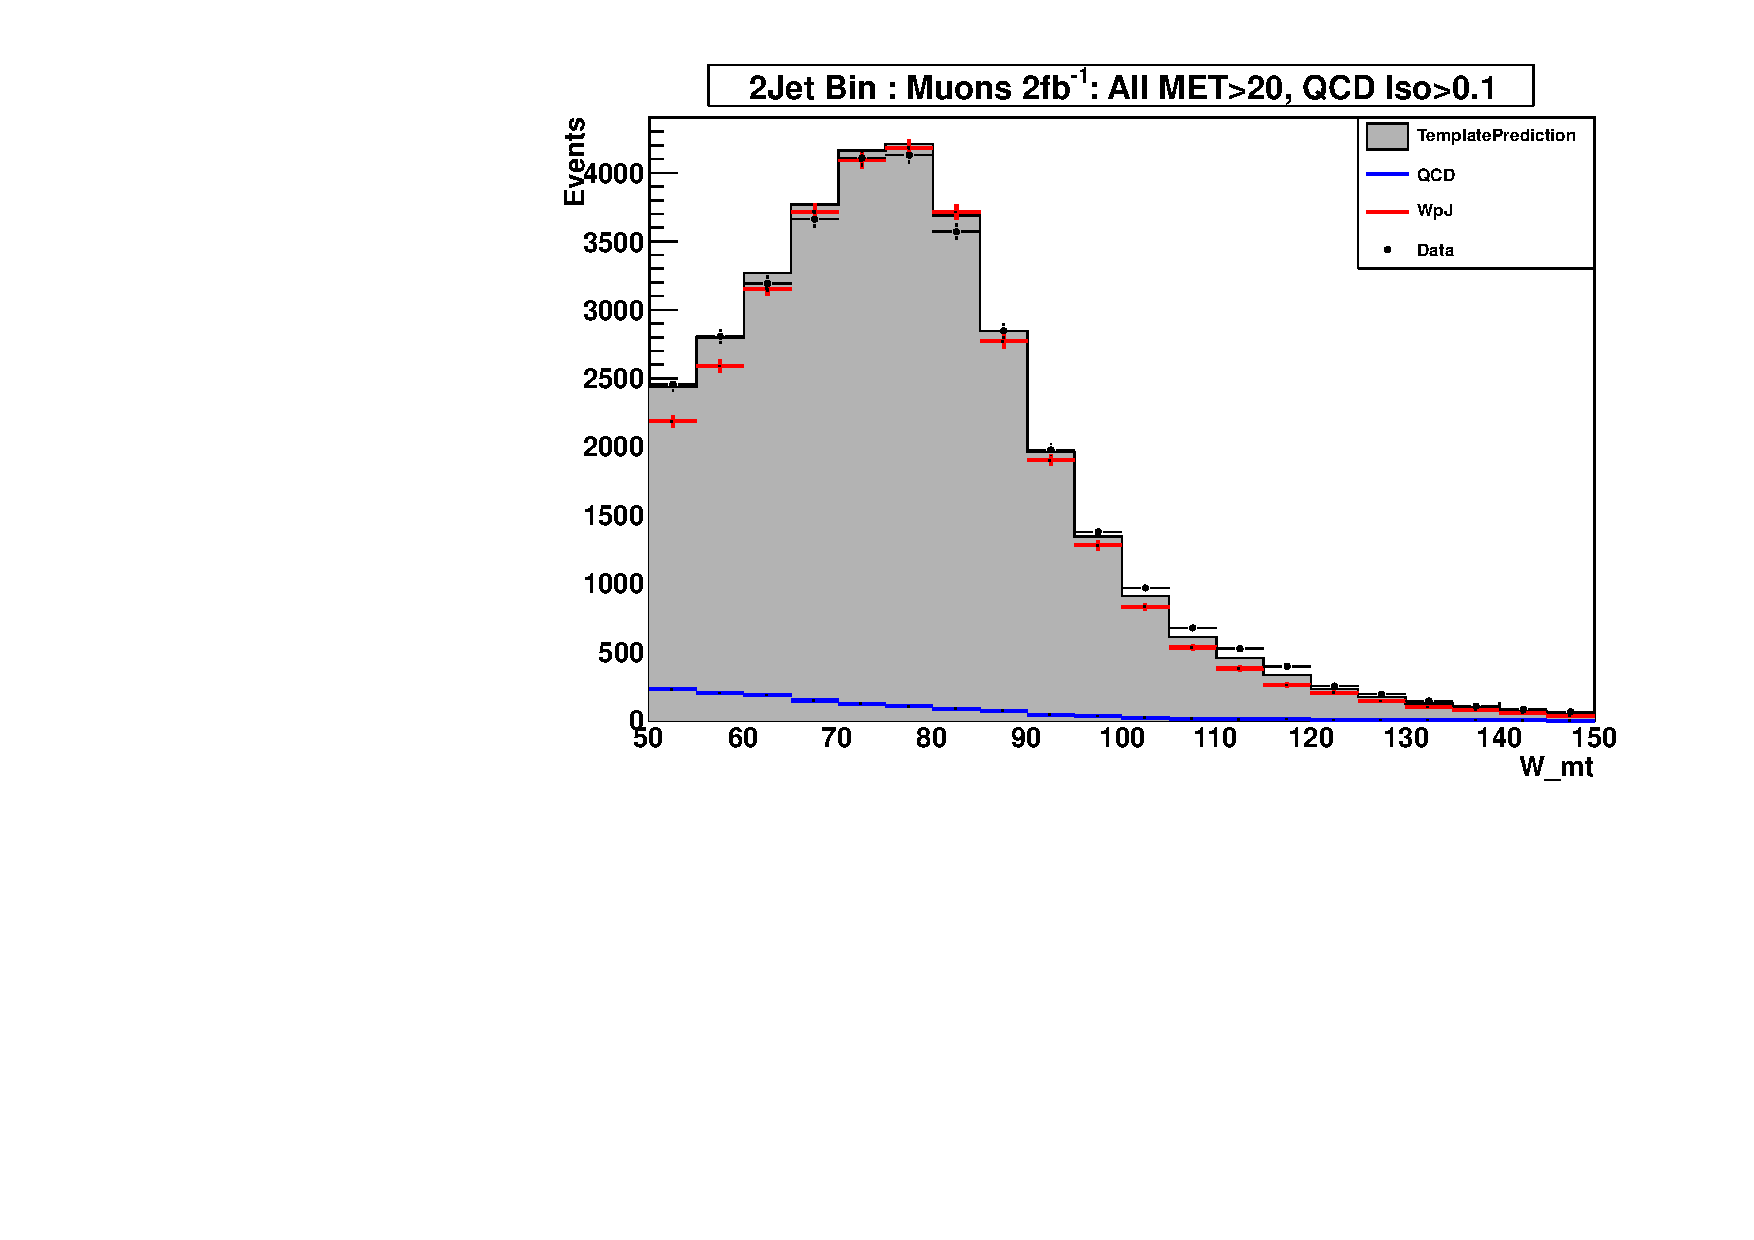
\includegraphics[width=0.48\textwidth]{figs/QCDFit2J_Muons_Isog01NoMETDataCuts.pdf}
%\put(-0.80,0.0){(a)} 
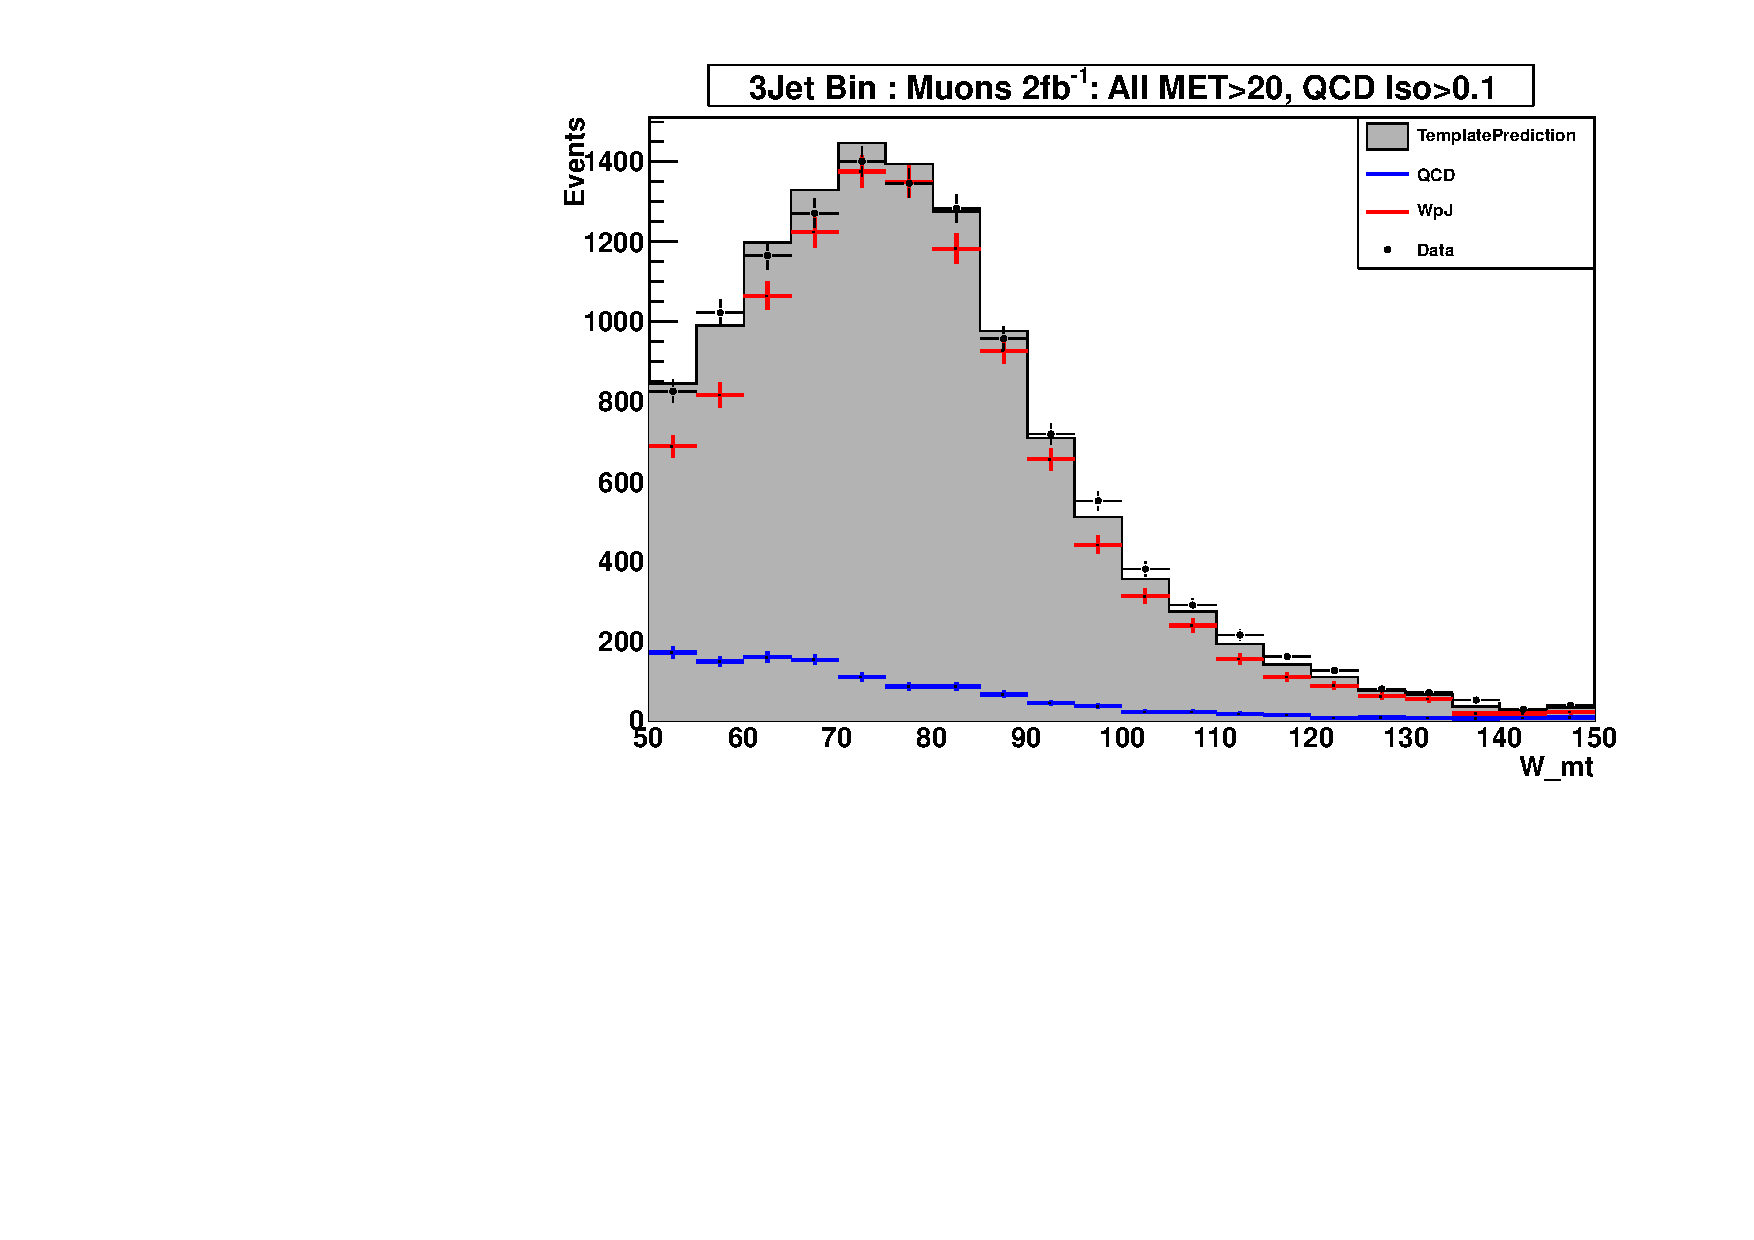
\includegraphics[width=0.48\textwidth]{figs/QCDFit3J_Muons_Isog01NoMETDataCuts.pdf}
%\put(-0.80,0.0){(b)} 
%\unitlength=0.33\linewidth
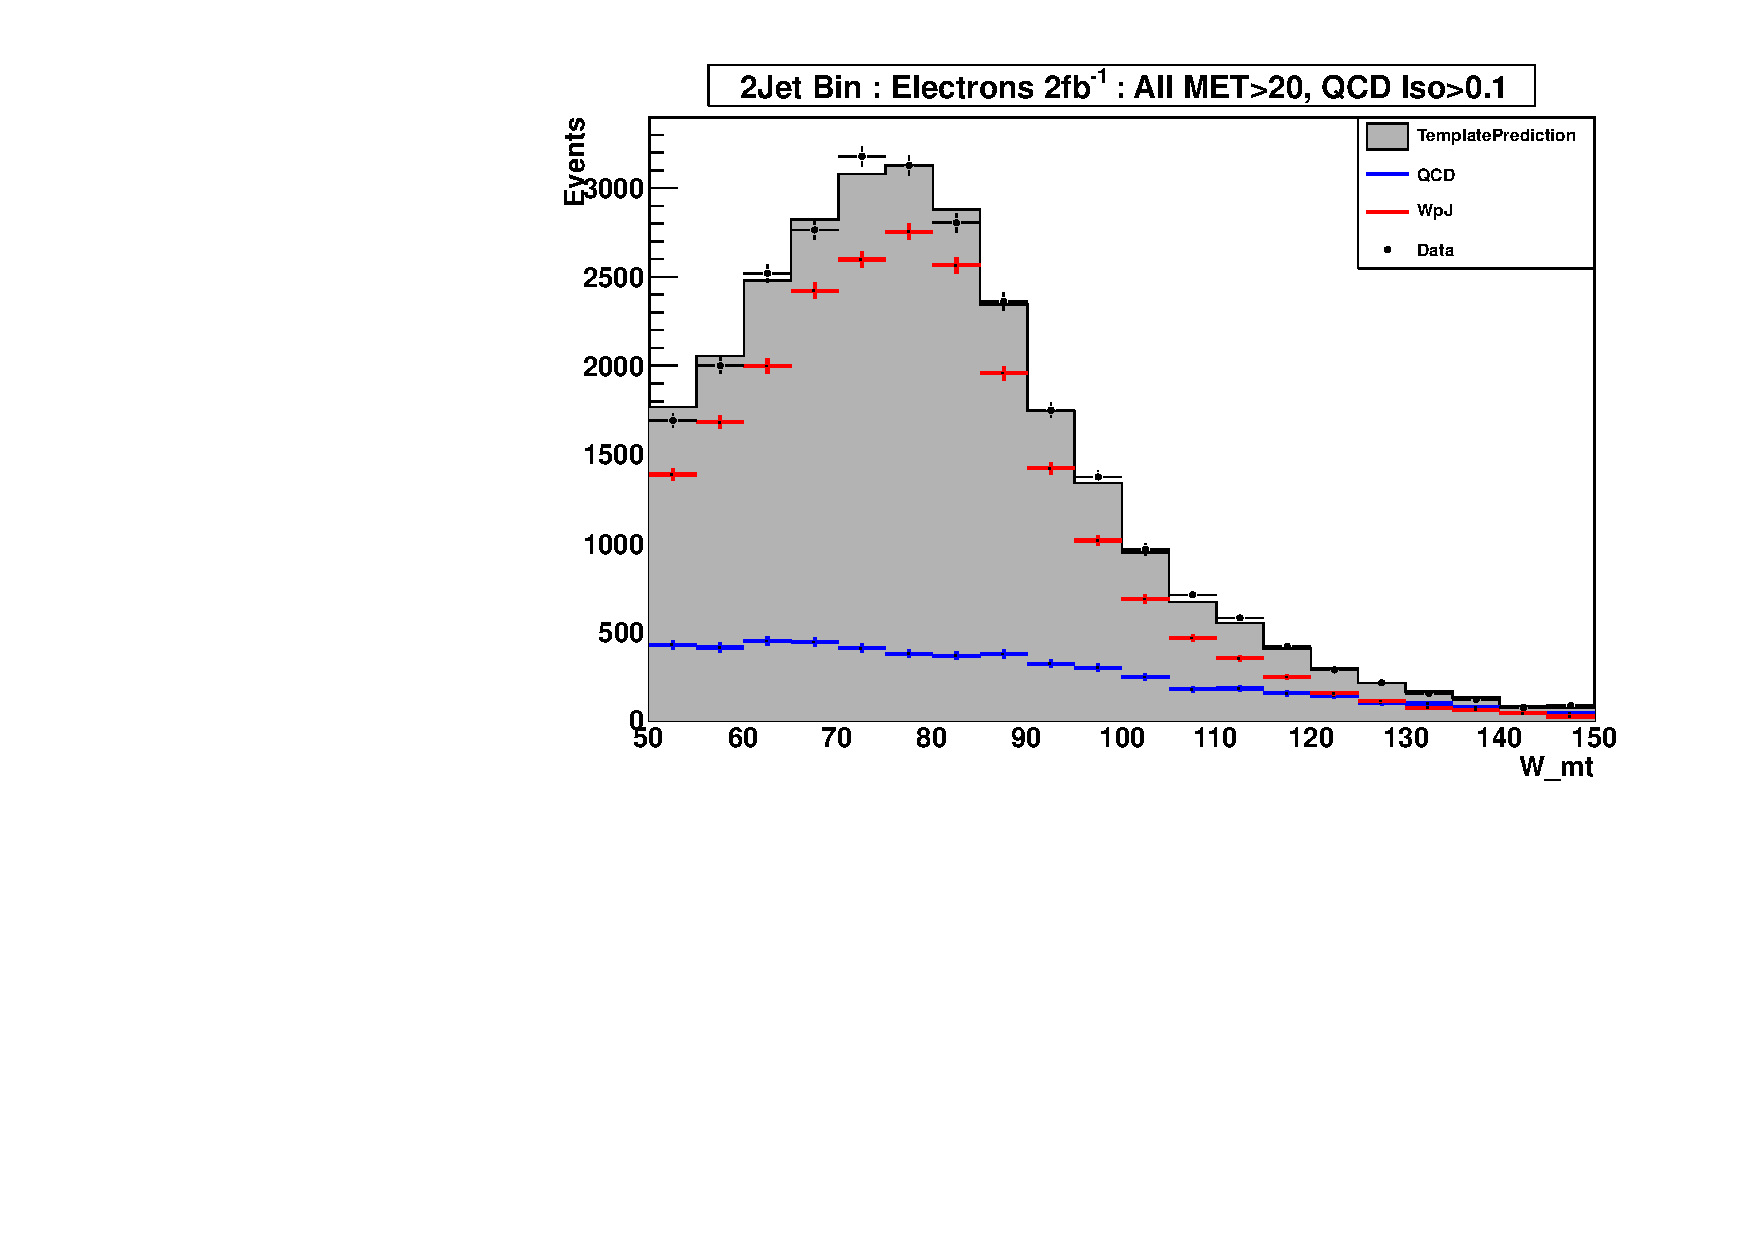
\includegraphics[width=0.48\textwidth]{figs/QCDFit2J_Electrons_Isog01NoMETDataCuts.pdf}
%\put(-0.80,0.0){(c)} 
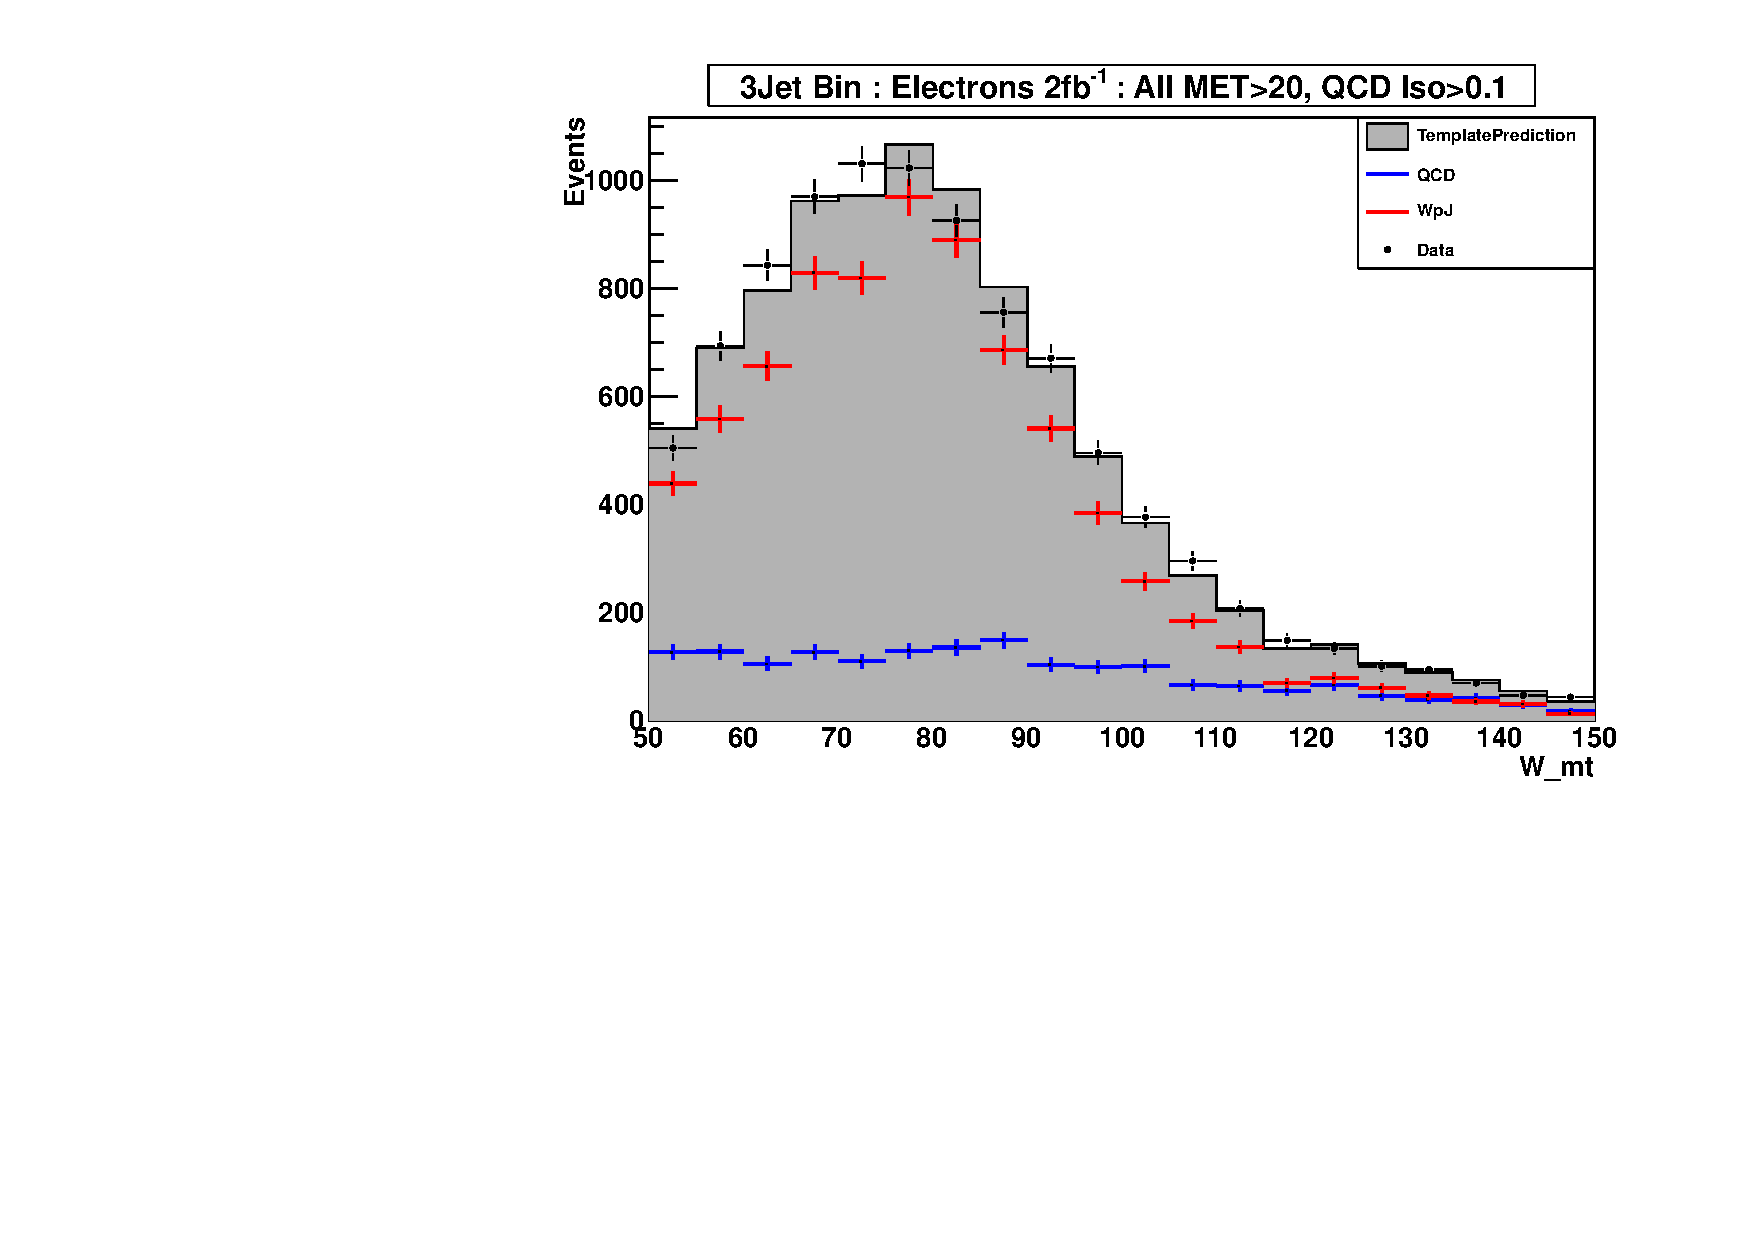
\includegraphics[width=0.48\textwidth]{figs/QCDFit3J_Electrons_Isog01NoMETDataCuts.pdf}
%\put(-0.80,0.0){(d)} 
\caption{$W_{mT}$ distributions fitted with QCD and W$jj$ templates in muon and electron data.} 
\label{fig:QCDTemplateFitWmT}}
\end{figure}
%%%%%%%
%%%%%%%%%%%%%%%%%%%%%%%%%%%%
